\chapter{Introduction}
\label{cha:intro}
This thesis contains all the work done to implement a tiny network stack for battery-free communication.\\
The microcontroller family used in this project is MSP430. These microcontrollers are built on a 16-bit processor that provides low power consumption.\\
Before looking in detail at what has been implemented, it is worthwhile to provide some background information to introduce the current situation of battery-free communication.\\
\section{Battery-Free Devices}
\label{sec:batteryFreeDevices}
The use of distributed sensors in the environment is a very interesting frontier for IoT applications; however, it is impossible to think of being able to wire all connections.\\
For this reason Wireless Sensor Networks (WSNs), distributed networks of sensors that communicate wirelessly, are being introduced.\\
In recent years processors are becoming less energivorous and batteries more durable but thinking about a sensor network that relies on batteries does not seem the best solution.
Batteries need to be replaced periodically \cite{BatteryDegradation}, and this is complicated if the nodes are in environments that are difficult or unsafe to reach.\\
To make the nodes energy-autonomous, researchers are working on systems that harvest energy from the environment in a capacitor to use as a power source; some examples of energy are solar \cite{7479815}, RF \cite{article} , kinetic \cite{KineticEnergy}, thermal \cite{ThermalEnergy} and some  bacteria species \cite{10.1145/3362053.3363491}.\\
In this way, there is no need to rely on batteries, and the system can work for its entire lifetime without \cite{ManteinanceWSN} or with minimal maintenance.\\
The energy harvested by these devices is employed to produce and get data from external sources, process it, and send it to other nodes in the network.\\
The operation of these devices is closely related to environmental conditions, and it is not guaranteed to always have sufficient energy to perform all the intended tasks. \\
Because of this low reliability of the energy level for task completion, nodes are prone to power failures and consequently work intermittently.\\ 
The frequency of these outages depends on many factors, such as capacitor size, available energy in the environment, and node consumption.\\
\section{Problem Statement}
\label{sec:problemStatement}
Stored energy is precious and should not be wasted. If a node transmits a packet and the receiving side does not have enough energy to finish receiving, the packet is lost, and there is a power failure on the node (Figure \ref{fig:TransmissionProblem}).
Power failures can have many other causes such as producing a data item without first verifying the availability of energy for proper production or suddenly consuming more energy than expected.
\\Anyway, in the event of a power failure, the node loses all the data it had produced and must consume more energy to produce the data again. At the same time, data received from other nodes in the network are lost. The latter scenario presents a considerable waste of energy; in fact, the energy used to produce, send and receive the packet is wasted.\\
To avoid these problems we need to:
\begin{enumerate}
\item Save data in non-volatile memory so that nothing is lost in case of power failure
\item Resume data management to just before power failure
\item Recognize expired data and delete them
\end{enumerate}
These problems must be solved in a way that provides the application layer with the methods of producing/sending and receiving data while hiding their complexity from the end user.
\begin{figure}[ht]
\centerline{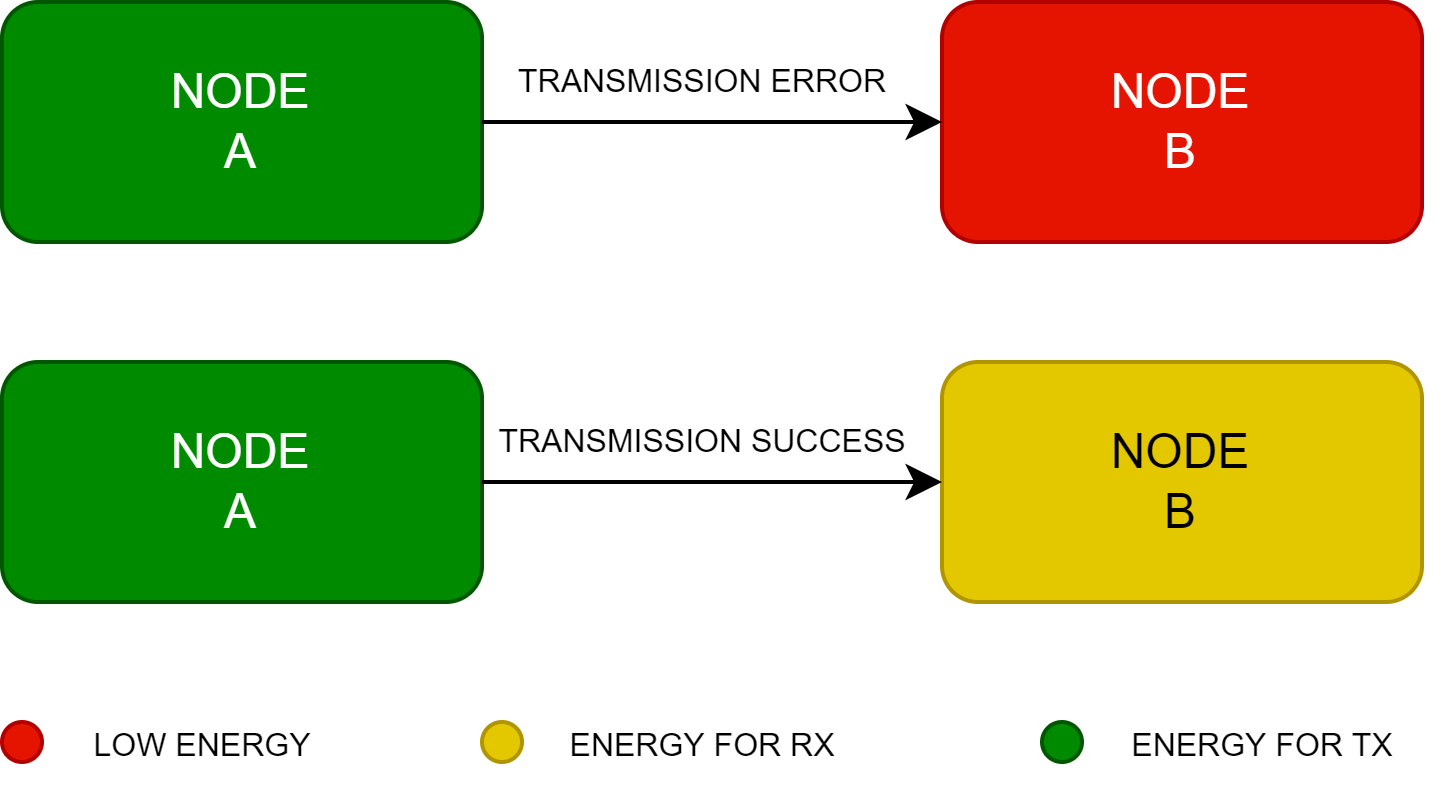
\psfig{file=Images/TransmissionProblem.png,width=0.6\textwidth}}
\caption{\footnotesize \centering Transmission examples}
\label{fig:TransmissionProblem}
\end{figure}
\section{Contributions}
\label{sec:contributions}
There are methodologies to limit power failures, such as the TRAP protocol \cite{9733918}, but it is impossible to be certain that they will not happen. Therefore, the contributions of this thesis are to present a Communication Stack for battery-free communication that:
\begin{enumerate}
\item Implements the TRAP protocol \cite{9733918} to be aware of the energy level of neighboring nodes
\item Saves data received from the Application Layer in non-volatile memory
\item Saves data received from the Physical Layer in non-volatile memory
\item Recovers data from memory in cases of power failure
\item Delete expired data to avoid unnecessary sending or processing
\item Send and receive data to and from Application Layer
\item Send and receive data to and from Physical Layer
\end{enumerate}
In addition to the problems that the stack aims to solve, we want a system that is modular and easily scalable.\\
In particular, the stack must be easily usable by the Application Layer and easily usable by the Physical Layer even when there are a large number of nodes in the network.\\
The Physical Layer must also not be binding on the stack, which must be able to work with different communication technologies, such as RF Backscatter communication \cite{transientComp} or VLC communication \cite{VLCCOmm}, by changing only the Physical Layer.\\
For these reasons, the nonfunctional requirements of the stack are:
\begin{itemize}
    \item Scalability
    \item Modularity
\end{itemize}
  

\newpage